% This is the entry point of the MLRC 2022 template
\documentclass{rescience}
% Place all your includes in the packages.tex file. Check the file for more information
% Place your include packages here

% IMPORTANT NOTES
% Please do not import xcolor, as rescience.cls already imports this package
% Please do not import "fontenc". ReScience uses custom fonts, which breaks when fontenc is loaded on top of it.
% Basically, DO NOT import the following:
% \usepackage[T1]{fontenc}

% If you face compilation issues, check our past commits in the editorial repository: https://github.com/ReScience/MLRC

% Some standard imports are done for you. Feel free to import more here
\usepackage{hyperref}       % hyperlinks
\usepackage{url}            % simple URL typesetting
\usepackage{booktabs}       % professional-quality tables
\usepackage{amsfonts}       % blackboard math symbols
\usepackage{nicefrac}       % compact symbols for 1/2, etc.
\usepackage{microtype}      % microtypography
\usepackage{multirow}
\usepackage{graphicx}
\usepackage{colortbl}
\usepackage{amsmath}
\usepackage{float}
\usepackage{booktabs}
\usepackage{xcolor}     

% Clever references
\usepackage[noabbrev,capitalize,nameinlink]{cleveref}
\crefformat{section}{\S#2#1#3}  % remove space between section symbol and the number
\crefname{section}{\S}{\S\S}
\Crefname{section}{\S}{\S\S}
\crefname{table}{Table}{}
\crefname{figure}{Figure}{}
\crefname{algorithm}{Algorithm}{}
\crefname{equation}{Equation}{}
\crefname{appendix}{Appendix}{}
\crefname{thm}{Theorem}{}
\crefname{prop}{Proposition}{}
\crefname{cor}{Corollary}{}
\crefname{observation}{Observation}{}
\crefname{assumption}{Assumption}{}
\crefformat{section}{\S#2#1#3}


\usepackage{multirow}

\usepackage{subcaption}
\usepackage{adjustbox}
\hypersetup{
    colorlinks=true,
    %urlcolor=cyan,   
    linkcolor=blue
}
\begin{document}
% DO NOT MODIFY THE CONTENTS OF header.tex
%% ----------------------------------------------------------------------------
%% ReScience article template
%% Copyright (c) 2018 N.P. Rougier,
%% Released under a Creative Commons Attribution 4.0 International license.
%% ----------------------------------------------------------------------------

%% --- Top left header --------------------------------------------------------
\begin{tikzpicture}[remember picture, overlay]
  \node [shape=rectangle, draw=darkred, fill=darkred, yshift=-34mm,
        anchor=north west, minimum width=3.75cm, minimum height=10mm]
        at (current page.north west) {};
  \node [text=white, anchor=center, yshift=-39mm, xshift=1.875cm]
         at (current page.north west) {\small \SpaceRoboto RESCIENCE C};
\end{tikzpicture}


%% --- Title -------------------------------------------------------------------
{\let\newpage\relax\maketitle} \maketitle


%% --- Margin information -----------------------------------------------------
\marginnote{
  \footnotesize \sffamily
  \textbf{Edited by}\\
  \ifdefempty{\editorNAME}{\textcolor{darkgray}{(Editor)}}
             {\editorNAME\ifdefempty{\editorORCID}{}{$^{\orcid{\editorORCID}}$}}\\
  ~\\
  %%
  \textbf{Reviewed by}\\
  \ifdefempty{\reviewerINAME}{\textcolor{darkgray}{(Reviewer 1)}}
             {\reviewerINAME\ifdefempty{\reviewerIORCID}{}{$^{\orcid{\editorORCID}}$}}\\
  \ifdefempty{\reviewerIINAME}{\textcolor{darkgray}{(Reviewer 2)}}
             {\reviewerIINAME\ifdefempty{\reviewerIIORCID}{}{$^{\orcid{\editorORCID}}$}}\\
  ~\\
  %%           
  \textbf{Received}\\
  \ifdefempty{\dateRECEIVED}{---}{\dateRECEIVED}\\
  ~\\
  %%
  \textbf{Published}\\
  \ifdefempty{\datePUBLISHED}{---}{\datePUBLISHED}\\
  ~\\
  %%
  \textbf{DOI}\\
  \ifdefempty{\articleDOI}{---}{\articleDOI}
}
 

%% --- Bottom statement -------------------------------------------------------
\newcommand{\container}[1]{\def\@container{#1}}
\begin{container}
  \afterpage {
    \begin{statement}
      \scriptsize \sffamily
      \hrule \vskip .5em
      Copyright © \articleYEAR~\authorsABBRV,
      released under a Creative Commons Attribution 4.0 International license.
      
      Correspondence should be addressed to
      \contactNAME~(\href{mailto:\contactEMAIL}{\contactEMAIL})
  
      The authors have declared that no competing interests exists.

      \ifdefempty{\codeURL}{}
      {Code is available at
      \href{\codeURL}{\codeURL}\ifdefempty{\codeDOI}{.}{ -- DOI \doi{\codeDOI}.}}

      \ifdefempty{\dataURL}{}
      {Data is available at
      \href{\dataURL}{\dataURL}\ifdefempty{\dataDOI}{.}{ -- DOI \doi{\dataDOI}.}}

      \ifdefempty{\reviewURL}{}
     {Open peer review is available at \href{\reviewURL}{\reviewURL}.}
    \end{statement}
  }
\end{container}


%% --- Abstract ---------------------------------------------------------------
%% \ifdefempty{\articleABSTRACT}{}{
%%   {\small \sffamily \textbf{Abstract} \articleABSTRACT \par}
%% }


%% --- Replication ------------------------------------------------------------
\ifdefempty{\replicationBIB}{}{
  {\small \sffamily \bfseries A replication of }
  \ifdefempty{\replicationURL}
       {\href{http://doi.org/\replicationDOI}{\small \sffamily \replicationBIB}}
       {\href{\replicationURL}{\small \sffamily \replicationBIB}}.
\par }


% IMPORTANT NOTE
% The title information should be added in metadata.yaml file. If you are compiling locally, then follow the instructions in https://github.com/ReScience/template. Else, you may edit the metadata.tex file directly. You can modify the fields "articleTITLE" and "articleABSTRACT".

% IMPORTANT NOTE: Ensure that you DO NOT ADD any author information, as that would violate double blind leading to desk rejection.


% Add the Reproducibility Summary in summary.tex
\section*{\centering Reproducibility Summary}

% \textit{Template and style guide to \href{https://paperswithcode.com/rc2022}{ML Reproducibility Challenge 2022}. The following section of Reproducibility Summary is \textbf{mandatory}. This summary \textbf{must fit} in the first page, no exception will be allowed. When submitting your report in OpenReview, copy the entire summary and paste it in the abstract input field, where the sections must be separated with a blank line.}

\subsubsection*{Scope of Reproducibility}

We reproduce the results in the paper Automatic Multi-Label Prompting: Simple and Interpretable Few-Shot Classification by Wang et al. \cite{Wang}. Using human prompt engineering can be long and expensive for text classification. In their paper they proposed an approach, called AMuLaP to do automatic label prompting for few-shot classification and claimed competitive performance on the GLUE benchmark. We reproduce their results on 3 GLUE datasets and extend them to 2 new datasets. 

\subsubsection*{Methodology}

We used the author's code with some additions to accommodate our new datasets and other models. We ran all experiments using a combination of hyperparameters given by the original authors over 5 seeds, mainly using RTX8000 for 125 hours.

\subsubsection*{Results}

We validate the original paper's claims by reproducing its metrics within the reported standard deviation, proving the method's competitiveness. Our extended trials highlight the method's potential applicability to real-world data and reveal new considerations about prompt template, language model, and seed for optimal performance.

\subsubsection*{What was easy}

The complete code implementation was available publicly with step-by-step instructions on how to get AMuLaP running with GLUE datasets. This made it easy to begin reproducing the work. Finding flagged and non-flagged tweets from Donald Trump to create our dataset was easy thanks to \url{thetrumparchive.com} which compiled this.

\subsubsection*{What was difficult}

The original code is lengthy and lacks information on implementation dependencies, making it time-consuming to understand. It is made only for GLUE tasks and RoBERTa models and needs modification to work on new experiments. Some language models are not built for mask completion, thus not directly suitable for AMuLaP, and required us to search for solutions extensively. Finally, as label engineering is also tied to prompt engineering, we find expanding the work through the template given in the code challenging without prior experience in manual prompt engineering.


\subsubsection*{Communication with original authors}

We did not feel the need to reach out to the authors as the method was well explained and simple to understand with basic probability knowledge and going through the code.

\newpage
% Add your paper contents in content.tex
%\textit{\textbf{The following section formatting is \textbf{optional}, you can also define sections as you deem fit.
%\\
%Focus on what future researchers or practitioners would find useful for reproducing or building upon the paper you choose.\\
%For more information of our previous challenges, refer to the editorials \cite{Sinha:2022,Sinha:2021,Sinha:2020,Pineau:2019}.
%}}
\section{Introduction}
Machine Learning models have shown great performance in multiple domains over the last decade. However, recent investigations into different real-world applications have shown that some models have bias in them and thus make unfair decisions \cite{mehrabi2021survey}. That is why algorithms have been created which provide high-confidence fairness guarantees \cite{agarwal2018, thomas2019}. Fairness in the context of decision-making is the absence of any prejudice or favoritism toward an individual or group based on their inherent or acquired characteristics, e.g. race or sex \cite{mehrabi2021survey}. However, current models don't take the potential probabilistic increase or decrease of subgroups in the deployment data into account. We call this phenomenon a \textit{demographic shift}. A demographic shift is a distribution change between the training and deployment distributions, which can be explained by a shift in the marginal distribution of a single random variable. This makes it not possible to guarantee high-confidence fairness for the current models. 
\newline
\newline
To address this issue, an algorithm has been created that provides the high-confidence guarantees that one or more user-specified fairness constraints will hold, despite a demographic shift between training and deployment without using data from the deployment environment \cite{giguere2022}. 


%A few sentences placing the work in high-level context. Limit it to a few paragraphs at most; your %report is on reproducing a piece of work, you don’t have to motivate that work.

\section{Scope of reproducibility}
\label{sec:claims}

The main contribution of the original paper \cite{giguere2022} is \textit{Shifty}, an algorithm which guarantees with high confidence that certain fairness constraints will hold even after a demographic shift occurs. This tackles the problem that the fairness guarantees of existing algorithms \cite{thomas2019, agarwal2018} do not hold when a demographic shift occurs upon deployment. \textit{Shifty} is designed to work in the following two scenarios: 

\begin{enumerate}
    \item The demographic proportions in the deployment population are known (known demographic shift).  
    \item The demographic proportions in the deployment population are bounded to known intervals (unknown demographic shift).
\end{enumerate}

\textit{Shifty} is widely applicable since it is model-agnostic, and accompanied by an open source-framework. When using \textit{Shifty}, the user can specify a fairness attribute, for which a certain fairness constraint should hold, and a demographic attribute, which may undergo demographic shift upon deployment. The following claims about \textit{Shifty} are made: 

\begin{enumerate}
    \item  \textit{Shifty} provides high-confidence fairness guarantees under demographic shifts.
    \item  Given that sufficient training data exists, \textit{Shifty} shows no loss in accuracy compared to other models.
    \item  If too little training data exists, or if the fairness constraints are not satisfied, \textit{Shifty} returns \textit{NSF} (No Solution Found).
    \item \textit{Shifty} is model-agnostic and can be used in combination with any classification model
\end{enumerate}

%The main contributions that are made by this paper are the following:

%\begin{enumerate}
%    \item Shifty is the first classification algorithm that provides high-confidence fairness guarantees under demographic shifts
%    \item A constructive proof of fairness guarantees is provided in the paper.
%    \item The algorithm is evaluated on and validated by real-world data.
%    \item An open-source implementation has been made so that other people can use Shifty as well.
%\end{enumerate} 

The goal of this paper is to test whether the claims made in the paper are reproducible, check whether \textit{Shifty} can be assumed to work in other domains and models as well, and to verify the reproducibility of the open-source implementation of the algorithm.

%The main contribution of the original article is \textit{Shifty}, a family of algorithms which guarantees which high confidence that certain fairness constraints will hold even after a demographic shift within certain bounds occurs.
% this tackles the problem that the fairness guarantees of existing algorithms do not hold when a demographic shift occurs upon deplyoment.

%Claims:
%\begin{itemize}
%    \item  shifty avoids bias under demographic shift, while existing methods do not
%    \item  returns no solution if insufficient training data or constraints are not satisfiable together (authors claim this does not happen often)
%    \item  no loss in accuracy if suffient data exists (unlike other models)
%\end{itemize}

%-----
%Introduce the specific setting or problem addressed in this work, and list the main claims from the original paper. Think of this as writing out the main contributions of the original paper. Each claim should be relatively concise; some papers may not clearly list their claims, and one must formulate them in terms of the presented experiments. (For those familiar, these claims are roughly the scientific hypotheses evaluated in the original work.)

%A claim should be something that can be supported or rejected by your data. An example is, ``Finetuning pretrained BERT on dataset X will have higher accuracy than an LSTM trained with GloVe embeddings.''
%This is concise, and is something that can be supported by experiments.
%An example of a claim that is too vague, which can't be supported by experiments, is %``Contextual embedding models have shown strong performance on a number of tasks. We will run experiments evaluating two types of contextual embedding models on datasets X, Y, and Z."

%This section roughly tells a reader what to expect in the rest of the report. Clearly itemize the claims you are testing:
%\begin{itemize}
%    \item Claim 1
 %   \item Claim 2
%    \item Claim 3
%\end{itemize}

%Each experiment in Section~\ref{sec:results} will support (at least) one of these claims, so a reader of your report should be able to separately understand the \emph{claims} and the \emph{evidence} that supports them.

%\jdcomment{To organizers: I asked my students to connect the main claims and the experiments that supported them. For example, in this list above they could have ``Claim 1, which is supported by Experiment 1 in Figure 1.'' The benefit was that this caused the students to think about what their experiments were showing (as opposed to blindly rerunning each experiment and not considering how it fit into the overall story), but honestly it seemed hard for the students to understand what I was asking for.}

\section{Methodology}
%Explain your approach - did you use the author's code, or did you aim to re-implement the approach from the description in the paper? Summarize the resources (code, documentation, GPUs) that you used.
The authors made their code repository publicly available on GitHub \cite{sgiguere2022github}. Unfortunately, the code from the repository produced numerous errors which we had to resolve in order to run the experiments.  Furthermore, we contributed by adding documentation, a complete environment file, result data conversion to the JSON format, and additional code to create figures, tables, and conduct statistical tests.


\subsection{\textit{Shifty} algorithm}

%Include a description of each model or algorithm used. Be sure to list the type of model, the number of parameters, and other relevant info (e.g. if it's pretrained). 
The \textit{Shifty} algorithm consists of three main parts: data partitioning, candidate selection and a fairness test.

\paragraph{Data partitioning} Initially, the data is split in two parts, one for candidate selection ($D_c$) and for for the fairness test ($D_f$). If the same dataset were to be used for both selecting a model and performing the fairness test, then the outcome of these two steps would be correlated. By ensuring that candidate selection and the fairness test use independent sets of observations this correlation is eliminated. This is necessary to guarantee that the overall algorithm satisfies property \textbf{A} (1) below.

%This ensures that the fairness does not "overfit" on the training data.

\paragraph{Candidate selection} This part involves training of the candidate model. Since this is not responsible for establishing the fairness guarantees, any existing classification algorithm can be used. As in the original paper, we use a linear classification model consisting of one linear layer with no bias term. The output which are produced by this linear layer are then passed through a sign function, which returns $-1$ for negative signs and $1$ for positive signs.

\paragraph{Fairness test} Given the candidate model from the previous step, \textit{Shifty} performs a fairness test by computing a high-confidence upper bound for every given fairness definition. If the upper bounds for the respective fairness definitions are all below zero, \textit{Shifty} returns the candidate model. Otherwise, \textit{No Solution Found (NSF)} is returned. The fairness test is based on one or multiple fairness definitions $g$, for which it holds that $g(\theta) > 0$ if and only if $\theta$ behaves unfairly.
If the candidate model is returned, it satisfies properties \textbf{A} and \textbf{B} for all fairness definitions $g$ shown in Equation \ref{eq:shiftyproperties} below. A model is considered fair with high confidence if property A is met.  Furthermore, $g'$ represent the fairness definitions after a demographic shift, used to evaluate Property \textbf{B}.

\begin{equation} \label{eq:shiftyproperties}
\text{\textbf{A)} } Pr(g(a(D)) \leq 0) \geq 1 - \delta \qquad \qquad \text{ \textbf{B)} } Pr(g'(a(D)) \leq 0) \geq 1 - \delta
\end{equation}
    
\subsection{Other fairness algorithms}
\textit{Shifty} is compared to three families of existing fairness algorithms: Fairness Constraints, Seldonian algorithms and Fairlearn, and finally RFLearn. Fairness Constraints provides fairness without guarantees, as opposed to Seldonian algorithms and Fairlearn which do provide high-confidence guarantees. Furthermore, RFLearn promotes fair outcomes under covariate shift without guarantees. \textit{Shifty} combines both, such that it provides fairness under demographic shift with a high-confidence guarantee. Every fairness algorithm has an implementation with a particular underlying classification and optimization method, which are summed up in Table \ref{table:models-compared}.

Interestingly, the Covariance Matrix Adaptation Evolution Strategy (\textit{CMA-ES}) is used for the optimization of the Seldonian algorithms and \textit{Shifty}, instead of the widely used and more efficient SGD. The reason that the authors opted out of using SGD might have to do with the fact that the fairness constraints are included in the loss functions for these algorithms. As a result, the loss function may be non-differentiable or difficult to differentiate. Therefore, CMA-ES is used since it is a derivative-free numerical optimization algorithm for non-convex problems. CMA-ES requires a lot more computations than SDG, so it will take significantly more time to train a model using CMA-ES as opposed to using SDG.

\begin{table}[H]
\centering
\begin{threeparttable}
\begin{tabular}{llll}
\toprule
{} &  Classification & Activation & Optimization \\
\midrule
Seldonian   & 1 linear layer, no bias  & sign function    & SLSQP + CMA-ES \\
FairConst   & 1 linear layer, no bias  & sign function    & SLSQP \\
Fairlearn   & linear SVC\tnote{1}      & n/a              & expgrad\tnote{2} \\
RFLearn     & 1 linear layer with bias & softmax function & SGD\tnote{3} \\
Shifty      & 1 linear layer, no bias  & sign function    & SLSQP + CMA-ES \\
\bottomrule
\end{tabular}

    \begin{tablenotes}
        \item[1] Support Vector Classifier
        \item[2] exponentiated gradient reduction
        \item[3] Stochastic Gradient Descent
    \end{tablenotes}

\end{threeparttable}
\caption{Overview of fairness models based on their classification, activation and optimization methods.}
\label{table:models-compared}
\end{table}


\subsection{Datasets}
\label{sec:datasets}
%For each dataset include 1) relevant statistics such as the number of examples and label distributions, 2) details of train / dev / test splits, 3) an explanation of any preprocessing done, and 4) a link to download the data (if available).
Two datasets were used for the experiments: The UCI Adult Census (Adult) dataset \cite{kohavi1996uci} and the UFRGS Entrance Exam and GPA (Brazil) dataset \cite{da2019ufrgs}. \\

\textbf{Adult dataset:} The Adult dataset includes various features and protected characteristic features like race and sex of 48,842 individuals taken during the 1994 US census. Just like the authors, we also considered a subset of the dataset corresponding to black or white individuals for running the experiments. The fairness attribute for this dataset is the race of an individual and the demographic attribute is the sex of an individual. The task used in this paper is to classify whether somebody`s income is above \$50,000 a year.\\
\textbf{Brazil dataset:} The Brazil dataset describes academic records for 43,303 students from a university in Brazil. For each student, the dataset includes a vector of entrance exam scores, their GPA, between 0 and 4, and the student’s race and sex. The fairness attribute for this dataset is the sex of an individual and the demographic attribute is the race of an individual. The task is to classify whether a student will have a GPA above 3, given their entrance exams scores.\\

For both classification tasks, the fairness and the demographic attribute are not taken into account when generating predictions, but solely to evaluate the models fairness. The original paper mentioned that the data was split evenly between $D_c$ and $D_f$. However in the code provided this split is 60\% - 40\%. For the experiments we stick to the values given in the code.

%In data preprocessing the adult dataset is adjusted so that it shows data consisting of only males with an income above 50,000.
%For the Brazil dataset preprocessing is done so that the data shows the students with their race and sex along with a GPA cutoff of above 3.0.

\subsection{Hyperparameters}
%Describe how the hyperparameter values were set. If there was a hyperparameter search done, be sure to include the range of hyperparameters searched over, the method used to search (e.g. manual search, random search, Bayesian optimization, etc.), and the best hyperparameters found. Include the number of total experiments (e.g. hyperparameter trials). You can also include all results from that search (not just the best-found results).
For the experiments we used the hyperparameters provided by the authors in  both the original paper and the code repository. However, certain hyperparameters found in the implementation did not match with what was stated in the paper, or were not given in the paper. In these cases we used the values provided in the original implementation.

\subsection{Experimental setup and code}
%Include a description of how the experiments were set up that's clear enough a reader could replicate the setup. Include a description of the specific measure used to evaluate the experiments (e.g. accuracy, precision@K, BLEU score, etc.). Provide a link to your code.

In order to run the original author's code, we needed to make some adjustments to the codebase. Our version of the repository is available at \url{\codeURL} and includes instructions on how to reproduce the experiments with the provided shell scripts or batch files. \\

To compare \textit{Shifty} with the other fairness algorithms, we trained every algorithm on both datasets with each of the following fairness definitions: disparate impact, demographic parity, equalized odds, predictive equality and equal opportunity. The formal definitions of these fairness definitions can be found in Appendix D2 of the original paper \cite{giguere2022}. To account for stochastic properties during the training process, we ran each experiment for the same number of trials as was specified in the original authors` implementation, which was either 25, 20, or 10 (specified in the shell script). Further, each experiment was run of sample sizes ranging between 10k and 60k, to investigate the algorithms sensibility to dataset size.
Performance and fairness of the models was compared by measuring their accuracy (\textit{Acc}) on the classification task, their proportion \textit{NSF}, and their \textit{Failure Rate (FR)}. The \textit{proportion NSF} represents the proportion of trials which did not return a solution, while \textit{FR} is the proportion of solutions which violated property \textbf{A} (original distribution) or property \textbf{B} (deployment distribution). The original authors specified the failure rate to be equal to $0$ when no solutions are found, but we changed this to \textit{n/a}, since stating that the failure rate is equal to $0$ when no solutions around in all cases does not represent the data well. \\


%Given the code, the virtual environment and the datasets we run the created batchfile which runs the code with the correct hyperparameters. The virtual environment can be installed using the YAML file provided in the code. The experiments where run on a multiple local machines and a LISA cluster. a LISA cluster is a compute cluster which consists of multiple nodes and clusters which allows the user to run computation-intensive tasks remotely rather than locally. To reproduce the experiments of authors, we measure the failure rates and accuracies of the different fairness models for multiple training sample sizes and fairness definitions. The fairness definitions we have evaluated are the following: disparate impact, demographic parity, equalized odds, predictive equality and equal opportunity. The formal definitions of these fairness definitions can be found in Appendix D2 of the original paper \cite{Giguere:2022}. \\

In addition to collecting and visualizing the experimental results, we performed two-sample t-tests on all trials which returned a solution, comparing the accuracy of \textit{Shifty} to the accuracy of the best model of the respective experimental run. This was done to verify the original author`s claim that Shifty performs at no loss of accuracy. Statistical significance was evaluated using a significance level $alpha = 0.05$ and as one comparison was made for each combination of fairness definition, dataset, and known/unknown bounds, Bonferroni correction was applied to prevent a family-wise increase in Type-I error. \\

Going beyond reproducing the experiments of the original paper, we investigated \textit{Shifty`s} sensibility to the size of the bounds limiting the unknown demographic shift. This was done by running \textit{Shifty} for multiple bound sizes on both classification tasks and for a dataset size of 60k samples. Further, to verify \textit{Shifty`s} usability with other optimizers than CMA-ES, we also ran experiments using the Broyden–Fletcher–Goldfarb–Shanno (BFGS) algorithm for optimization. This optimization method was already implemented by the original author, even though not being reported on in the original paper. Due to extensive running time we only applied the fairness definitions disparate impact and demographic parity for both of these extensions.

\subsection{Computational requirements}

\begin{table}[H]
\centering
\begin{tabular}{llll}
\toprule
CPU & RAM & \% of trials & Runtime (h)\\
\midrule
Apple M1, 8 cores              & 32 GB  & 18.75\% & 21 \\
Intel i7-11850H, 8 cores       & 16 GB  & 31.25\% & 21 \\
Intel i9-12900KF, 8 cores      & 32 GB  & 25\%    & 34 \\
Intel Xeon Gold 5118, 12 cores & 200 GB & 25\%    & 13 \\
\bottomrule
\end{tabular}
\caption{Overview of machines used to run the experiments and their corresponding runtimes. The percentage of trials only serves as an indication for the relative usage of each machine; the trials vary in datasets and parameters, so they are not identical.}
\label{table:runtime}
\end{table}

In order to run all the experiments from the original paper \cite{giguere2022}, we divided the workload across multiple machines. Table \ref{table:runtime} gives an overview of the machines we have used and their corresponding runtimes. In total, it took us $89$ hours of computation time to run all the experiments.

% Include a description of the hardware used, such as the GPU or CPU the experiments were run on. 
% For each model, include a measure of the average runtime (e.g. average time to predict labels for a given validation set with a particular batch size).
% For each experiment, include the total computational requirements (e.g. the total GPU hours spent).
% (Note: you'll likely have to record this as you run your experiments, so it's better to think about it ahead of time). Generally, consider the perspective of a reader who wants to use the approach described in the paper --- list what they would find useful.

\section{Results}
\label{sec:results}
% Start with a high-level overview of your results. Do your results support the main claims of the original paper? Keep this section as factual and precise as possible, reserve your judgement and discussion points for the next "Discussion" section. 


\subsection{Results reproducing original paper}
% For each experiment, say 1) which claim in Section~\ref{sec:claims} it supports, and 2) if it successfully reproduced the associated experiment in the original paper. 
% For example, an experiment training and evaluating a model on a dataset may support a claim that that model outperforms some baseline.
% Logically group related results into sections. 

% \begin{enumerate}
%     \item  \textit{Shifty} is the first classification algorithm that provides high-confidence fairness guarantees under demographic shifts.
%     \item  Given that sufficient training data exists, \textit{Shifty} shows no loss in accuracy compared to other models.
%     \item  If too little training data exists, or if the fairness constraints are not satisfied, \textit{Shifty} returns \textit{NSF} (No Solution Found).
%     \item \textit{Shifty} is model agnostic and can be used in combination with any classification model
% \end{enumerate}

Our results very much resemble the results achieved by the original author, while our statistical analysis highlights that in most cases, \textit{Shifty} performs significantly worse than the best model on the respective classification task. Tables \ref{diadult} and \ref{dibrazil}, as well as Figures \ref{fig:labelfreeadult} and \ref{fig:labelfreebrazil}, show the results for both datasets using disparate impact as a fairness definition, while additional results with different fairness definitions can be found in \ref{addoriginal}. Over all experiments, the proportion \textit{NSF} returned by \textit{Shifty} ranges between 0.125 and 1. $\Delta Acc$ refers to  the difference in classification accuracy between using a dataset of 10k and 60k samples. If no single solution could be found for 10k samples, this value is $n/a$. It is relevant to note that \textit{Shifty's} FR is always 0, while this is not the case for the comparison models.

\begin{table}[H]
\begin{threeparttable}
\centering
\begin{tabular}{lrrrrrrrr}
\toprule
 & \multicolumn{4}{c}{Known DS} & \multicolumn{4}{c}{Unknown DS} \\
 & NSF & Acc & FR & $\Delta$ Acc & NSF & Acc & FR & $\Delta Acc$ \\
\cmidrule(r){2-5} \cmidrule{6-9}
FairConst & n/a & 0.782 & 1.000 & -0.004 & n/a & 0.802 & 1.000 & -0.009 \\
RFLearn & n/a & \bfseries 0.787 & 1.000 & 0.000 & n/a & 0.823 & 1.000 & 0.005 \\
Fairlearn & n/a & 0.781 & 1.000 & -0.001 & n/a & \bfseries 0.842 & 1.000 & 0.007 \\
Quasi-SC & 0.520 & 0.762 & 0.417 & 0.111 & 0.600 & 0.767 & 0.500 & 0.139 \\
Shifty & 0.720 & 0.750\tnote{1} & \bfseries 0.000 & 0.074 & 0.400 & 0.750\tnote{2} & \bfseries 0.000 & 0.167 \\
SC & 0.680 & 0.759 & \bfseries 0.000 & 0.105 & 0.500 & 0.781 & \bfseries 0.000 & 0.140 \\
\bottomrule
\end{tabular}
\begin{tablenotes}
\item[1] significantly worse than best model, $p<0.001$, $t=12.987$, $df=30$
\item[2] significantly worse than best model, $p<0.001$, $t=32.561$, $df=24$
\end{tablenotes}
\end{threeparttable}
% \caption{Disparate Impact - adult dataset}
\caption{Comparison between the models for the greatest sample size using the Disparate Impact fairness definition and Adult dataset. Shifty differs significantly from the best performing model, and fewer solutions are found. For the first three models NSF is not applicable, since there is always a solution returned. \textit{DS} = Demographic Shift, \textit{NSF} = No Solution Found, \textit{Acc} = Accuracy, \textit{FR} = Failure Rate, $\Delta$ \textit{Acc} = Difference in accuracy between the largest and smallest sample size.}
\label{diadult}
\end{table}



\begin{table}[H]
\begin{threeparttable}
\centering
\begin{tabular}{lrrrrrrrr}
\toprule
 & \multicolumn{4}{c}{Known DS} & \multicolumn{4}{c}{Unknown DS} \\
 & NSF & Acc & FR & $\Delta$ Acc & NSF & Acc & FR & $\Delta$ Acc \\
\cmidrule(r){2-5} \cmidrule{6-9}
FairConst & n/a & 0.612 & 1.000 & -0.001 & n/a & 0.612 & 1.000 & 0.001 \\
RFLearn & n/a & 0.648 & 0.040 & -0.001 & n/a & 0.642 & \bfseries 0.000 & -0.004 \\
Fairlearn & n/a & 0.650 & 0.600 & -0.001 & n/a & 0.649 & 0.600 & 0.000 \\
Quasi-SC & 0.000 & \bfseries 0.657 & 0.400 & 0.008 & 0.000 & \bfseries 0.656 & 0.200 & 0.007 \\
Shifty & 0.600 & 0.606\tnote{1} & \bfseries 0.000 & 0.130 & 0.450 & 0.480\tnote{2} & \bfseries 0.000 & 0.030 \\
SC & 0.000 & 0.657 & 0.240 & 0.010 & 0.050 & 0.654 & \bfseries 0.000 & 0.009 \\
\bottomrule
\end{tabular}
\begin{tablenotes}
\item[1] significantly worse than best model, $p<0.001$, $t=5.357$, $df=33$
\item[2] significantly worse than best model, $p<0.001$, $t=22.643$, $df=29$
\end{tablenotes}
\end{threeparttable}
\caption{Comparison between the models for the greatest sample size using the Disparate Impact fairness definition and Brazil dataset. Shifty differs significantly from the best performing model, and fewer solutions are found.}
\label{dibrazil}
\end{table}

%The results for unknown demographic shift (antag) are similar for the Brazil dataset. \textit{Shifty} returns mostly \textit{NSF}, while the accuracy of the models which did have a solution, stay relatively the same. The case is different for the Adult dataset. The amount of \textit{NSF} cases are smaller and the accuracy is relatively higher.

\clearpage

\begin{figure*}[h]
    \centering
    \begin{subfigure}[b]{1\linewidth}
        \includegraphics[width=\textwidth]{img/charts/adult/fixed/iclr_adult_demographic_shift_sex_di.png}
    \end{subfigure}
    \begin{subfigure}[b]{1\linewidth}
        \includegraphics[width=\textwidth]{img/charts/iclr_legend.png} 
    \end{subfigure}
    \caption{The results when enforcing disparate impact constraints on the UCI Adult Census dataset under known demographic shift}\label{fig:labelfreebrazil}
\end{figure*}

\vspace{-20pt}

\begin{figure*}[h]
    \centering
    \begin{subfigure}[b]{1\linewidth}
        \includegraphics[width=\textwidth]{img/charts/adult/antag/iclr_adult_demographic_shift_sex_di.png}
    \end{subfigure}
    \begin{subfigure}[b]{1\linewidth}
        \includegraphics[width=\textwidth]{img/charts/iclr_legend.png} 
    \end{subfigure}
    \caption{The results when enforcing disparate impact constraints on the UCI Adult Census dataset under unknown demographic shift}
\label{fig:labelfreeadult}
\end{figure*}


%For demographic parity the \textit{NSF} probability reduces as the number of training examples grows. Both results are worse when compared with the results reported by the original paper. Interestingly, our result when applying disparate impact as a fairness constraint returns all \textit{NSF} which is different than what the authors claimed in their paper: namely, that \textit{Shifty} producing a \textit{NSF} is rare.


%\vspace{1em}
%\textbf{Known demographic shift:} We evaluated the performance of the fairness algorithms, with known and unknown demographic shifts. We found that when When we run the code with a fixed demographic shift, we see that for the Brazil dataset, \textit{Shifty} returns a solution in less than 10\% of all cases. For the Adult dataset, \textit{Shifty} returns \textit{NSF} 30\% and 66\% of the time for the unknown and known demographic shifts respectively. 

\subsection{Results beyond original paper}
% Often papers don't include enough information to fully specify their experiments, so some additional experimentation may be necessary. For example, it might be the case that batch size was not specified, and so different batch sizes need to be evaluated to reproduce the original results. Include the results of any additional experiments here. Note: this won't be necessary for all reproductions.

\subsubsection{Bound size of unknown demographic shift} Figure \ref{fig:bounds} displays how \textit{Shifty`s} performance and proportion \textit{NSF} change when the size of the bounds defining the possible demographic shift change. A general trend can be seen that as the bounds become larger, classification accuracy decreases and the proportion \textit{NSF} increases. 

\begin{figure}[H]
\centering
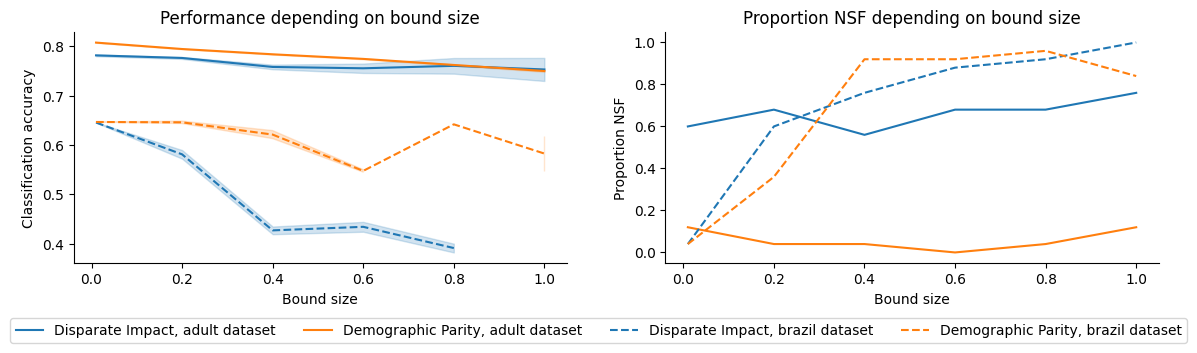
\includegraphics[width=\textwidth]{img/charts/Bounds.png}
\caption{\textit{Shifty`s} performance and proportion  NSF when demographic shift is limited to bounds of certain size. The shaded area represents the standard error.}
\label{fig:bounds}
\end{figure}

\subsubsection{Comparing different optimizers with \textit{Shifty}}  We have used three different optimization methods using the \textit{Shifty} implementation: CMA-ES (default), BFGS and linear-shatter. Linear-shatter turned out to be impractical, because the computation time was too high. Therefore, a comparison between only CMA-ES and BFGS is shown in Table \ref{diadultoptimizer}. We notice that the accuracy is slightly worse overall for BFGS. Furthermore, we have measured that BFGS leads to a runtime which is roughly 2x the runtime of CMA-ES. Additional results for this experiment can be found in Appendix \ref{addbeyond}.

\begin{table}[H]
\centering
\begin{tabular}{lrrrrrrrr}
\toprule
 & \multicolumn{4}{c}{Known DS} & \multicolumn{4}{c}{Unknown DS} \\
 & NSF & Acc & FR & $\Delta$ Acc & NSF & Acc & FR & $\Delta$ Acc \\
\cmidrule(r){2-5} \cmidrule{6-9}
CMA-ES & 0.720 & \bfseries 0.750 & \bfseries 0.000 & 0.074 & 0.400 & \bfseries 0.750 & \bfseries 0.000 & 0.167 \\
BFGS & 0.440 & 0.724 & \bfseries 0.000 & 0.073 & 0.600 & 0.725 & \bfseries 0.000 & 0.210 \\
\bottomrule
\end{tabular}
\caption{Comparison between CMA-ES and BFGS optimization methods for the \textit{Shifty} implementation using the UCI Adult Census dataset and the Disparate Impact fairness definition.}
\label{diadultoptimizer}
\end{table}


\section{Discussion}
% Give your judgement on if your experimental results support the claims of the paper. Discuss the strengths and weaknesses of your approach - perhaps you didn't have time to run all the experiments, or perhaps you did additional experiments that further strengthened the claims in the paper.

The reproduced results support the claims made by the authors to a large extent: (1) By design, \textit{Shifty} guarantees that the fairness guarantees even hold under demographic shift, which the results confirm as \textit{Shifty} never violated these constraints upon deployment. (2) The claim that, given sufficient data, \textit{Shifty} performs at no loss of accuracy compared to other models does not hold in all problem settings. In almost all cases in which \textit{Shifty} returned a sufficient number of solutions to conduct statistical analysis, it performed significantly worse than the best model, and when applying disparate impact as a fairness definition on the Brazil dataset, \textit{Shifty} even performed worse than random with an accuracy of 0.48 for the unknown demographic shift setting and with the largest dataset size. As for some problem settings \textit{Shifty`s} accuracy is comparable to the other models, it would be necessary to evaluate on a case-by-case basis if the trade-off between loss of accuracy and fairness guarantees is worth it.
%For some fairness constraints there was an insufficient number of solutions for Shifty to viably compare it to the best performing model, but for the cases in which comparison was possible, the loss is indeed minor. This trade-off can be worth the additional value of guaranteed fairness. 
(3) As again guaranteed by design, \textit{Shifty} reliably returns \textit{NSF} when it cannot guarantee the specified constraints with the data given. However, the results show that this happens more often than claimed, and sometimes even up to 100\% of the cases. Our additional experiments showed that this proportion \textit{NSF} is dependent on the size of the bounds limiting the unknown demographic shift, and it would be a valuable future research question to investigate how other hyper-parameters influence the proportion \textit{NSF}. (4) While \textit{Shifty} is model-agnostic by design, the original experiments did not verify this empirically as they were all run using CMA-ES. By comparing CMA-ES with BFGS, we have verified that both optimizers give comparable results, with BFGS being consistently worse than CMA-ES.

Unfortunately, the validity of the claims made is weakened by a few experimental aspects. Different methods were used to train the model parameters of \textit{Shifty} and the comparison models, using different amounts of computational resources and model structures. As these aspects can account for differences in performance, it makes it difficult to draw final conclusions about \textit{Shifty}. For example, Table \ref{table:models-compared} shows that the fairness models have differences in the underlying classification and optimization methods, which can impact the final accuracy of the model. \\

%Furthermore, the experiments on unknown demographic shift were predicting the possible demographic shift using interpolation. This does not allow us to conclude how \textit{Shifty} would perform when bounds were predicted by using domain knowledge, and to which extent the size of these bounds influences the performance of \textit{Shifty}. \\

Given that the claims would hold, another limitation of \textit{Shifty} may be its practicality when being applied to real-world problems. Since it already requires ~60,000 training examples to approach competitive performance when only training a one-layer model, it may not always be feasible to obtain enough labelled data to train more complex models. The relation between model performance, model complexity, and dataset size for \textit{Shifty} may be a valuable future research question. Further, while \textit{Shifty} in theory works with any classification model, it may not often find a solution when not incorporating the model`s fairness into the loss function. However, no implementation of \textit{Shifty} for popular optimization methods like Stochastic Gradient Descent (SGD) exists yet.

\subsection{What was easy}
% Give your judgement of what was easy to reproduce. Perhaps the author's code is clearly written and easy to run, so it was easy to verify the majority of original claims. Or, the explanation in the paper was really easy to follow and put into code. 

% Be careful not to give sweeping generalizations. Something that is easy for you might be difficult to others. Put what was easy in context and explain why it was easy (e.g. code had extensive API documentation and a lot of examples that matched experiments in papers).
The provided theory for the \textit{Shifty} algorithm, along with the proof was helpful in understanding the algorithm thoroughly. The original paper provided a lot of additional information in the appendix for better understanding. This was helpful in not only better understanding the code, but also to verify certain functions in the implementation.\\

Once the code was functional, the process of running the code and getting the results was straightforward. The authors  provided a batch file with multiple command lines to run the various experiments. With this batch file the necessary functions along with the given hyperparameters were successfully run after only a few adjustments.



\subsection{What was difficult}
% List part of the reproduction study that took more time than you anticipated or you felt were difficult. 

% Be careful to put your discussion in context. For example, don't say "the maths was difficult to follow", say "the math requires advanced knowledge of calculus to follow". 

\textbf{Understanding the implementation:}
During the project, we experienced difficulties understanding the implementation provided by the authors. The open-source code implementation for the \textit{Shifty} algorithm and the accompanying experiments was of significant size. The codebase consisted of about 15,000 lines of Python code lacked documentation, a large part of it was not relevant to the published paper, and a lack of structure made it difficult to extract the relevant material. What additionally contributed to the size and complexity of the codebase was that many code snippets were present at multiple locations in parts of the code. Fortunately, this redundancy can be fixed by defining generalized functions. Unfortunately, this was not a feasible task to accomplish during this project due to the limited time we had and the  size of the codebase. Furthermore, many relevant training aspects such as hyperparameters were hard-coded and difficult to find. These aspects also made it challenging to expand on the given implementation.
%Due to the limited time we had to initially divide parts of the codebase in order for us to get a complete understanding of the code that we were running. 
%\\
%We experienced the most difficulties with the implementation. Not much (detailed) explanation or reasoning where provided for certain functions and code parts. The code seemed unstructured, there were lots of code parts which where not used at all, redundant code was used multiple times and relevant training aspects were difficult to find. So the need of (proper) documentation for the implementation was really felt when we experienced these difficulties. Given these difficulties it resulted in another challenge which is to build upon this code and try to extend and improve the implementation. It is difficult to build upon a work if we are not able to properly understand the implementation.
The overall provided setup for the implementation failed in our case since the requirements file was not complete and additional bugs were present in the code. Furthermore, the given requirements and batch file could only be run on a Windows machine. Certain adjustments were done on our part in order to run the code on all the necessary local machines. \\

Finally, we noticed certain deviations between specifications made in the paper and their implementations in the codebase. For instance, the original paper stated that the data was evenly split (the code had a 60-40 split), 25 trials were run for all experiments (the code ran some experiments for only 20 or 10 trials), and interpolation factors of 0.25 and 0.3 were used (the code provided used 0.25 and 0.5). This created confusion in which specifications to apply for the experiments. Because we used the code provided by the authors we decided to give preference to the specifications in the codebase. \newline

\textbf{Comparing results:} An important aspect of our work was to reproduce the paper´s results with the setup provided by the authors. However, they only provided visualizations rather than the raw results, which made it difficult to engage in a precise comparison. 


\subsection{Communication with original authors}
% Document the extent of (or lack of) communication with the original authors. To make sure the reproducibility report is a fair assessment of the original research we recommend getting in touch with the original authors. You can ask authors specific questions, or if you don't have any questions you can send them the full report to get their feedback before it gets published. 
We contacted the first author of the original paper at the beginning of the second week, for instance, to ask for the raw values used for the visualizations in the paper. As of February 3rd, we have not received a response to our email. 


%At the beginning of the second week of the project, we sent a mail to the first author of the paper, Stephen Giguere, for certain questions we had. We asked whether we could receive the raw data he generated in order to compare it to the results we got. As of yet, Giguere still has to respond to our mail.

\hypersetup{linkcolor=black,urlcolor=darkgray}
\renewcommand\emph[1]{{\bfseries #1}}
\setlength\bibitemsep{0pt}
\printbibliography

% If you have appendix to add, add it in the appendix.tex file
\section{Appendix} \label{sec:appendix}

\subsection{\textit{UFRGS Entrance Exam and GPA} dataset}\label{sec:appendix1}

The following section contains the results considering the second dataset used for reproduction of the original experiments as described in section \ref{sec:datasets} and \ref{sec:experiments}. In this dataset sex is used as the fairness attribute, and race as the demographic attribute. 

The hyperparameters values used for these experiments are summarised in Table \ref{tab:brazil_hyperparams}.

\begin{table}[ht]
\centering
\footnotesize
    \begin{tabular}{l|c|c|c|c|c|c}
    Constraint & $\epsilon$ & train / test & Dc / Df & n-iters & $\delta$ & $\alpha$* \\\hline 
    DI & -0.8 & 0.4 & 0.4 &  2000 & 0.05 & 0.25\\
    DP & 0.1 & 0.4 & 0.4 & 2000 & 0.05 & 0.25 \\
    \end{tabular}
    \caption{Hyperparameter values for the experiments run with the \textit{UFRGS GPA} dataset specified for Disparate Impact (DI) or Demographic Parity (DP) for both a known and unknown demographic shift. $\alpha$ is only used in the case of an unknown shift.}
    \label{tab:brazil_hyperparams}
\end{table}

Shown in figure \ref{fig:brazil_k_shift} are the results under a known demographic shift with DP and DI as the fairness constraints. Results under unknown demographic shift considering DP and DI as the fairness constraints are shown in figure \ref{fig:brazil_unk_shift}.

\begin{figure}[ht]
    \begin{subfigure}{\linewidth}
      \centering
      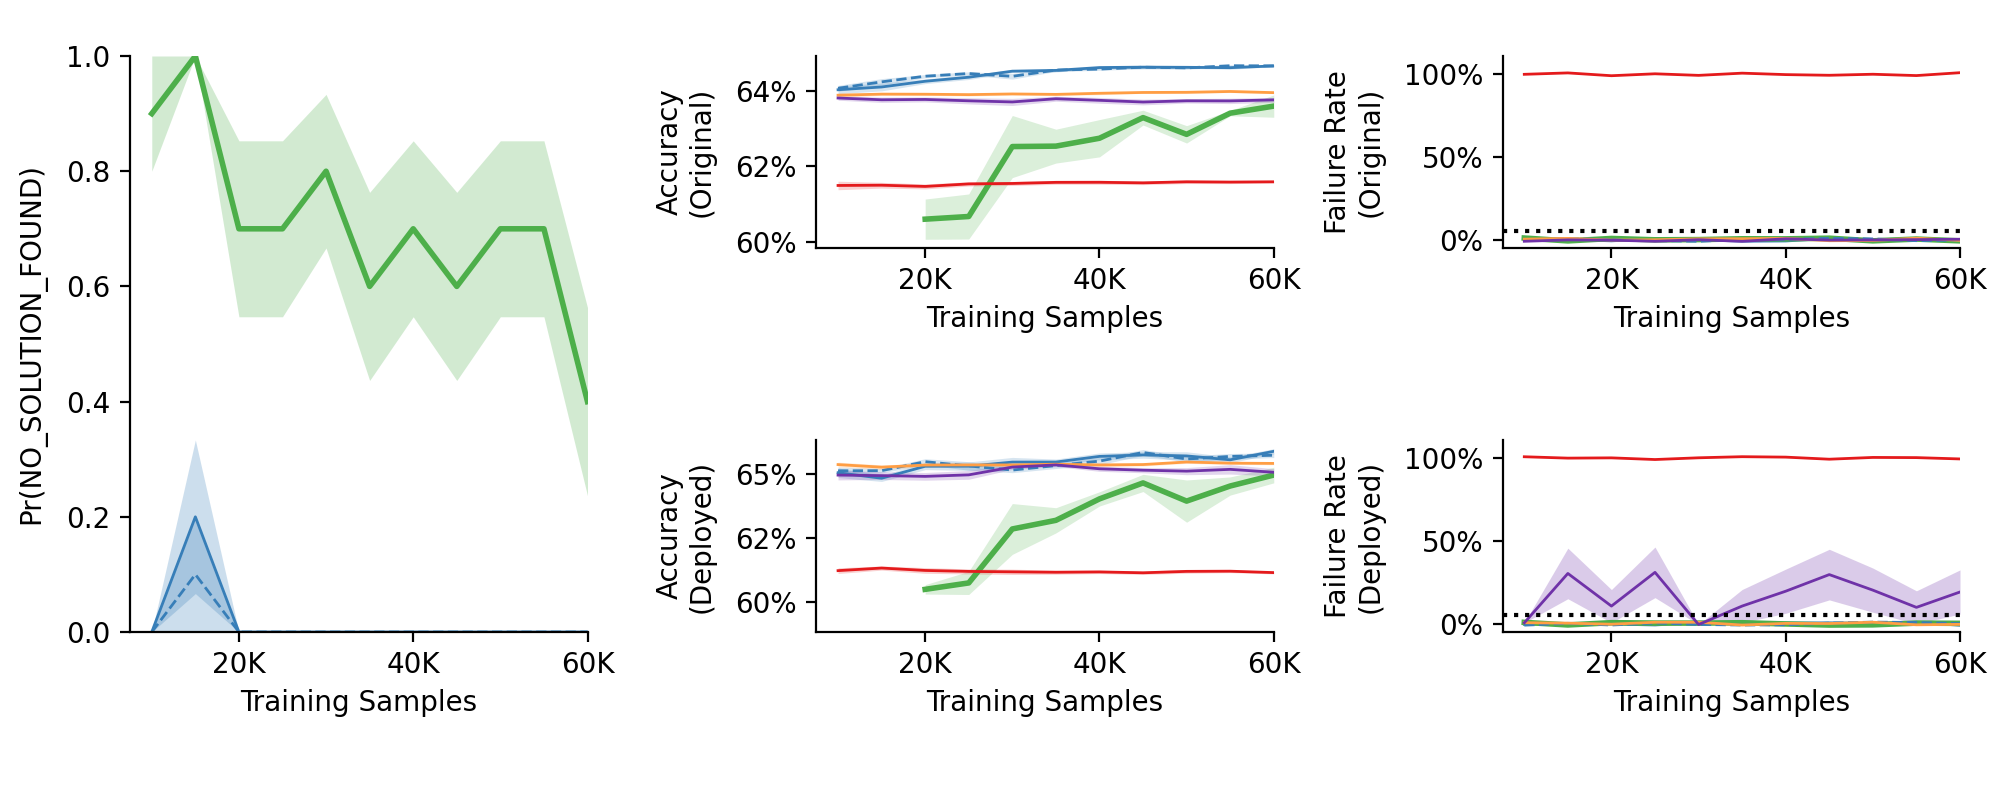
\includegraphics[scale=0.5]{figures/iclr_fixed_demographic_shift_brazil_rl/iclr_brazil_fixed_ds_rl_dp.png}
      \caption{Demographic Parity}
      \label{fig:brazil_k_dp}
    \end{subfigure}
    \begin{subfigure}{\linewidth}
      \centering
      \includegraphics[scale=0.5]{figures/iclr_fixed_demographic_shift_brazil_rl/iclr_brazil_fixed_ds_rl_di.png}
      \caption{Disparate Impact}
      \label{fig:brazil_k_di}
    \end{subfigure}
    \begin{subfigure}{\textwidth}
        \includegraphics[width=\linewidth]{figures/iclr_antag_demographic_shift_brazil_rl/iclr_legend.png}
    \end{subfigure}
    
    \caption{Results when enforcing fairness constraints under known demographic shift using the \textit{UFRGS GPA} dataset. For both fairness constraints DP and DI, the leftmost graph shows the probability of \texttt{NO\_SOLUTION\_FOUND}, the middle column shows the accuracies, and the rightmost column shows the failure rates.}
    \label{fig:brazil_k_shift}
\end{figure}



\begin{figure}[ht]
    \begin{subfigure}{\linewidth}
      \centering
      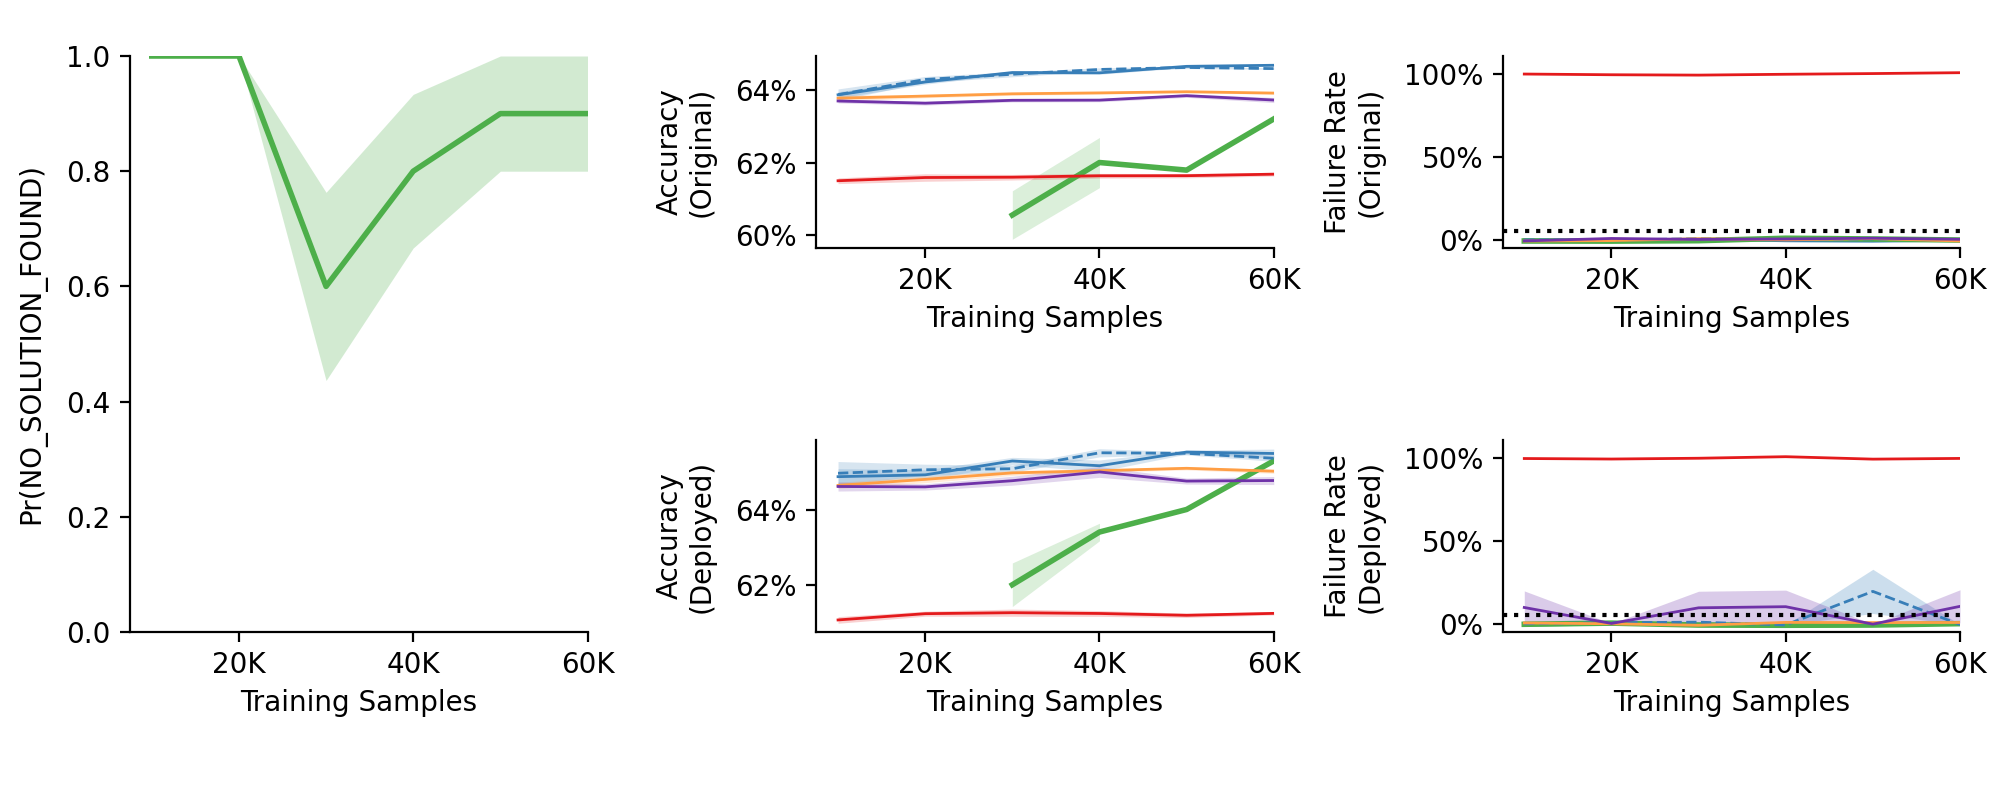
\includegraphics[scale=0.5]{figures/iclr_antag_demographic_shift_brazil_rl/iclr_brazil_antag_ds_rl_dp.png}
      \caption{Demographic Parity}
      \label{fig:brazil_unk_dp}
    \end{subfigure}
    \begin{subfigure}{\linewidth}
      \centering
      \includegraphics[scale=0.5]{figures/iclr_antag_demographic_shift_brazil_rl/iclr_brazil_antag_ds_rl_di.png}
      \caption{Disparate Impact}
      \label{fig:brazil_unk_di}
    \end{subfigure}
    \begin{subfigure}{\textwidth}
    \includegraphics[width=\linewidth]{figures/iclr_antag_demographic_shift_brazil_rl/iclr_legend.png}
    \end{subfigure}
    
    \caption{Results when enforcing fairness constraints under unknown demographic shift using the \textit{UFRGS GPA} dataset. For both fairness constraints DP and DI, the leftmost graph shows the probability of \texttt{NO\_SOLUTION\_FOUND}, the middle column shows the accuracies, and the rightmost column shows the failure rates.} 
    \label{fig:brazil_unk_shift}
\end{figure}

\subsection{\textit{UCI - Adult Census} Failure Rates} \label{sec:failure_rates_appendix}
In this section, the failure rates for each algorithm with the \textit{UCI Adult Census} dataset, as mentioned in section \ref{sec:discussion_fail}, are provided in Figures \ref{fig:adult_fr_unk} and \ref{fig:adult_fr_k}.

\begin{figure}[!h]
    \begin{subfigure}{0.5\linewidth}
      \centering
      \includegraphics[width=\linewidth]{figures/adult_failure_rates/iclr_adult_antag_ds_rl_dp.png}
      \caption{Demographic Parity}
    \end{subfigure}
    \begin{subfigure}{0.5\linewidth}
      \centering
      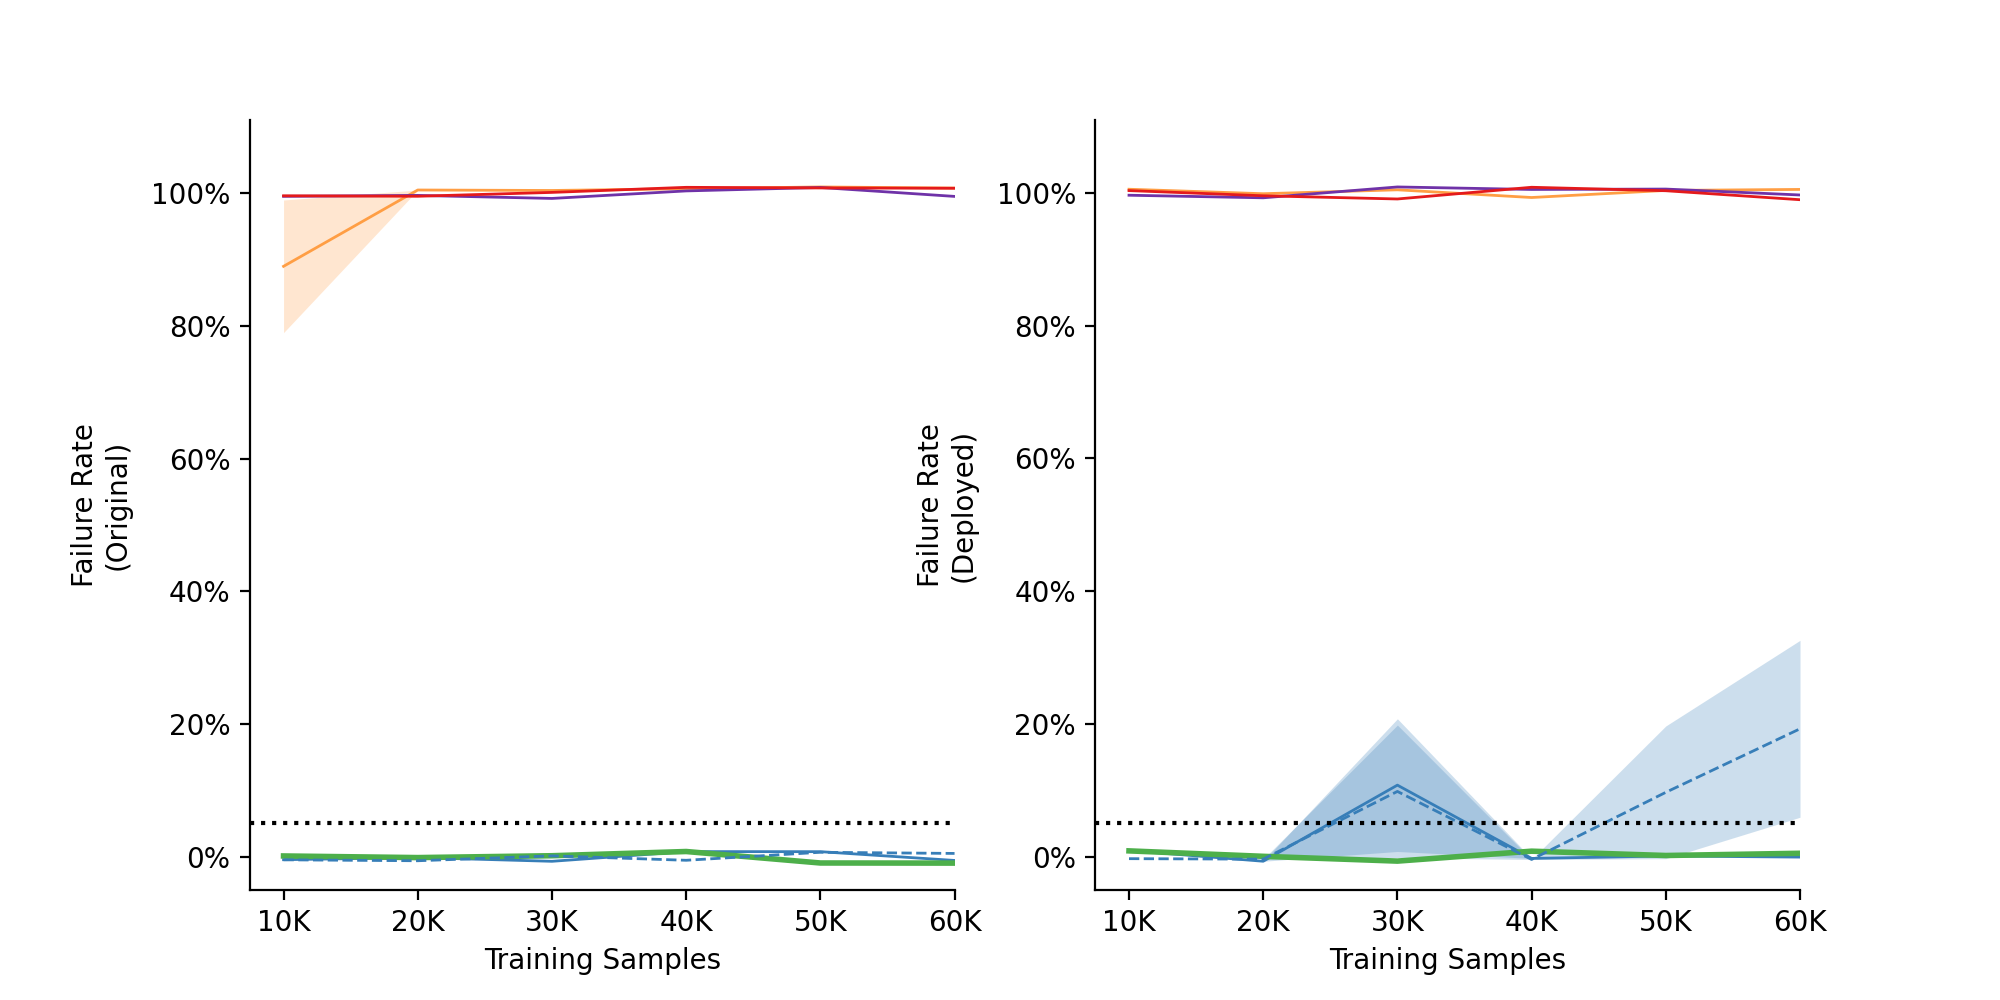
\includegraphics[width=\linewidth]{figures/adult_failure_rates/iclr_adult_antag_ds_rl_di.png}
      \caption{Disparate Impact}
    \end{subfigure}
    \begin{subfigure}{\textwidth}
    \includegraphics[width=\linewidth]{figures/adult_failure_rates/iclr_legend.png}
    \end{subfigure}
    \caption{Failure rates for each algorithm under unknown demographic shift for fairness constraints DP and DI with the \textit{UCI Adult Census} dataset. The confidence bound is indicated with the dotted line.} 
    \label{fig:adult_fr_unk}
\end{figure}


\begin{figure}[ht]
    \begin{subfigure}{0.5\linewidth}
      \centering
      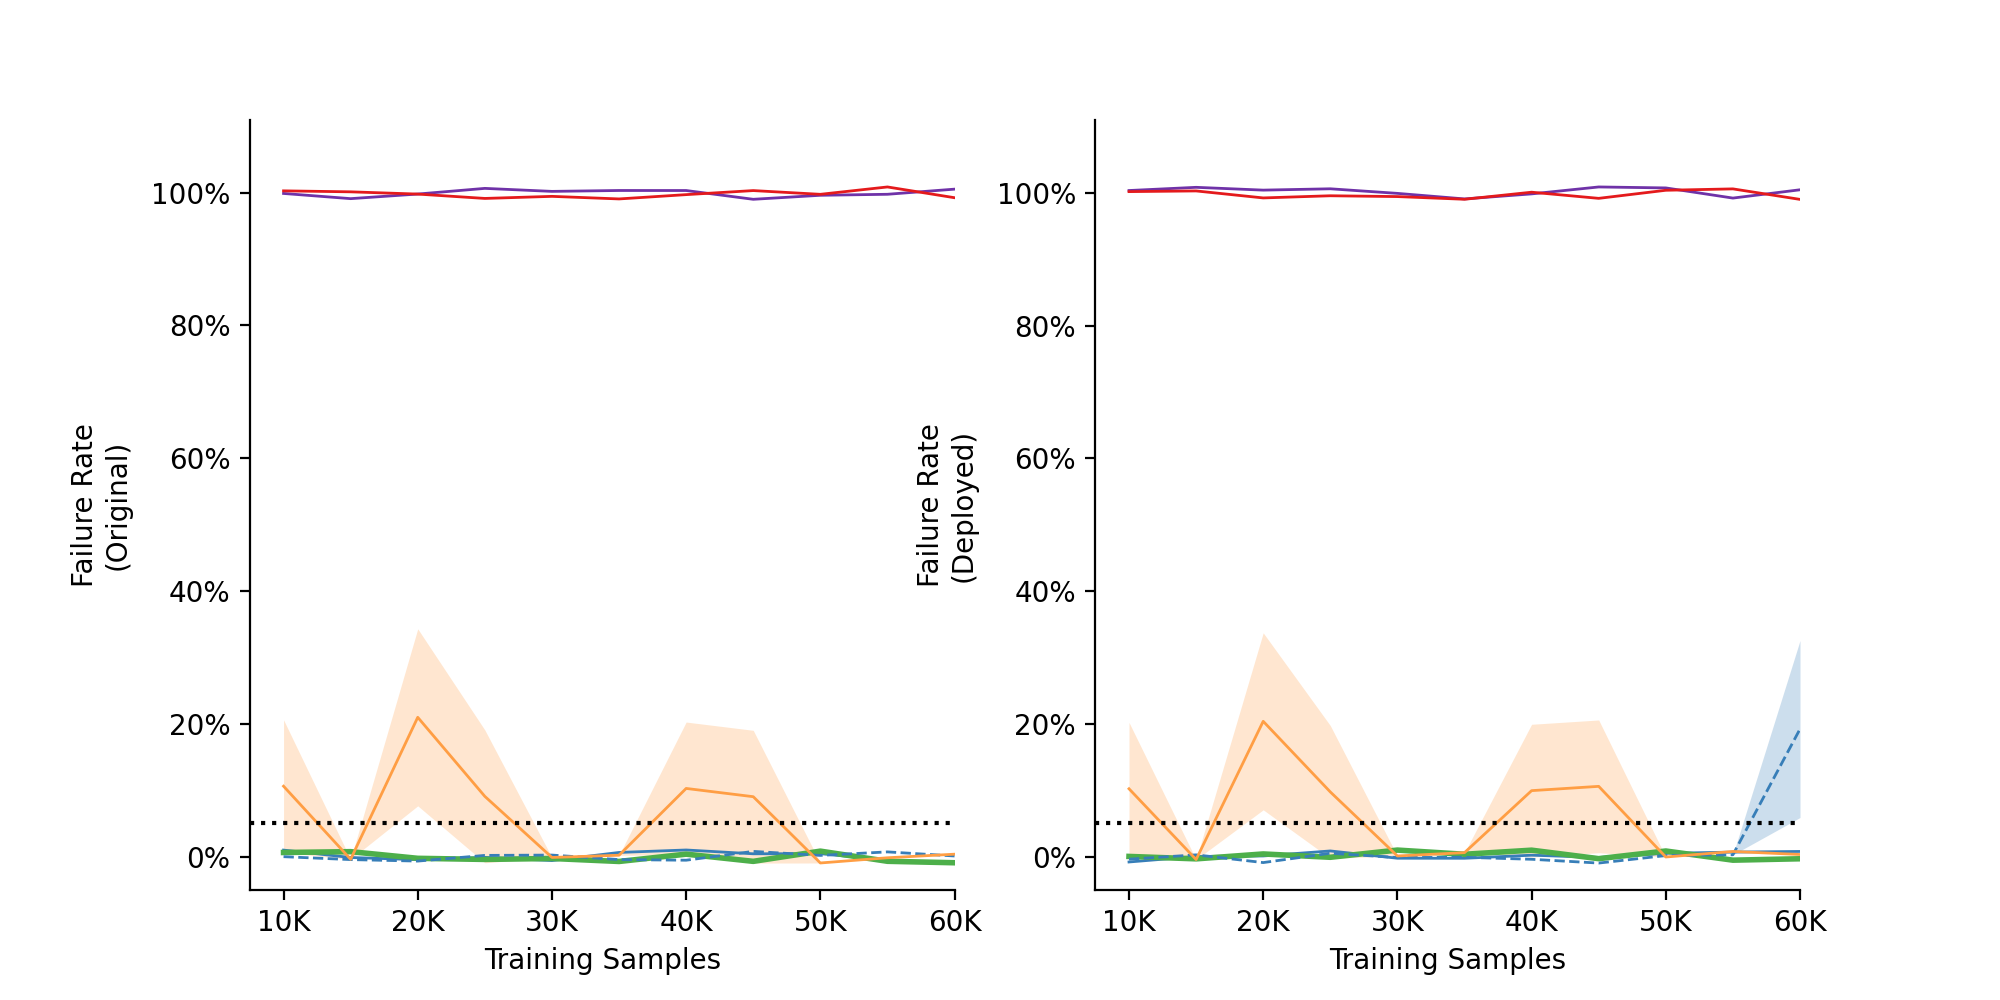
\includegraphics[width=\linewidth]{figures/adult_failure_rates/iclr_adult_fixed_ds_rl_dp.png}
      \caption{Demographic Parity}
    \end{subfigure}
    \begin{subfigure}{0.5\linewidth}
      \centering
      \includegraphics[width=\linewidth]{figures/adult_failure_rates/iclr_adult_fixed_ds_rl_di.png}
      \caption{Disparate Impact}
    \end{subfigure}
    \begin{subfigure}{\textwidth}
    \includegraphics[width=\linewidth]{figures/adult_failure_rates/iclr_legend.png}
    \end{subfigure}
    \caption{Failure rate (in percentages) for each algorithm under known demographic shift for fairness constraints DP and DI with the \textit{UCI Adult Census} dataset. The confidence threshold is indicated with the dotted line.} 
    \label{fig:adult_fr_k}
\end{figure}

\subsection{Numerical Results}\label{sec:app_num_results}
The tables in this section (tables \ref{tab:uci_num_k_DP}, \ref{tab:uci_num_k_DI}, \ref{tab:uci_num_unk_DP}, and \ref{tab:uci_num_unk_DI}) provide numerical results of the accuracy scores on the experiments run with the \textit{UCI Adult Census} dataset, as set out in section \ref{sec:discussion_accuracy}.
\begin{table}[ht] 
\footnotesize 
\begin{tabular}{|c|ccccccccccc|} \hline \multicolumn{12}{|c|}{Accuracy - Known Demographic Shift - Demographic Parity} \\ \hline \hline

Samples & 10k & 15k & 20k & 25k & 30k & 35k & 40k & 45k & 50k & 55k & 60k \\ \hline

\multicolumn{12}{|c|}{Seldonian Classifier} \\ \hline
Original & nan & nan & 76.05 & nan & 76.31 & 76.59 & 76.59 & 77.75 & 78.05 & 78.11 & 78.19 \\ \hline
Deployed & nan & nan & 72.80 & nan & 74.15 & 75.30 & 74.72 & 75.58 & 75.98 & 76.06 & 76.05 \\ \hline 
Difference & nan & nan & -3.25 & nan & -2.16 & -1.29 & -1.87 & -2.17 & -2.07 & -2.05 & -2.14 \\ \hline

\multicolumn{12}{|c|}{Quasi-Seldonian-Robust Classifier (\textbf{\texttt{Shifty}})} \\ \hline
Original & 76.75 & 76.25 & 77.17 & 77.56 & 77.34 & 77.80 & 77.91 & 77.99 & 77.99 & 77.93 & 77.95 \\ \hline
Deployed & 73.60 & 74.11 & 74.37 & 74.99 & 74.66 & 75.19 & 75.62 & 75.44 & 75.53 & 75.72 & 75.73 \\ \hline
Difference & -3.15 & -2.14 & -2.80 & -2.57 & -2.68 & -2.61 & -2.29 & -2.55 & -2.46 & -2.21 & -2.22 \\ \hline

\multicolumn{12}{|c|}{Quasi-Seldonian Classifier} \\ \hline
Original & 76.70 & 77.03 & 77.38 & 78.10 & 78.31 & 78.56 & 78.20 & 78.56 & 78.68 & 78.81 & 78.86 \\ \hline
Deployed & 73.47 & 74.35 & 74.56 & 75.70 & 75.96 & 76.60 & 75.66 & 76.43 & 76.42 & 76.67 & 76.69 \\ \hline
Difference & -3.23 & -2.68 & -2.82 & -2.40 & -2.35 & -1.96 & -2.54 & -2.13 & -2.26 & -2.14 & -2.17 \\ \hline

\multicolumn{12}{|c|}{Fairlearn} \\ \hline
Original & 74.03 & 74.39 & 74.78 & 74.11 & 74.36 & 74.40 & 74.13 & 74.15 & 74.41 & 74.40 & 74.43 \\ \hline
Deployed & 70.91 & 71.24 & 71.76 & 71.04 & 71.23 & 71.25 & 71.05 & 71.06 & 71.25 & 71.25 & 71.26 \\ \hline
Difference & -3.12 & -3.15 & -3.02 & -3.07 & -3.13 & -3.15 & -3.08 & -3.09 & -3.16 & -3.15 & -3.17 \\ \hline 

\multicolumn{12}{|c|}{RFLearn} \\ \hline
Original & 80.99 & 81.03 & 81.01 & 80.92 & 81.05 & 81.00 & 81.03 & 81.04 & 81.12 & 81.02 & 80.98 \\ \hline
Deployed & 78.51 & 78.55 & 78.56 & 78.46 & 78.56 & 78.52 & 78.58 & 78.59 & 78.68 & 78.59 & 78.53 \\ \hline Difference & -2.48 & -2.48 & -2.45 & -2.46 & -2.49 & -2.48 & -2.45 & -2.45 & -2.44 & -2.43 & -2.45 \\ \hline

\multicolumn{12}{|c|}{Fair Constraints} \\ \hline
Original & 80.99 & 80.77 & 80.71 & 80.63 & 80.60 & 80.58 & 80.64 & 80.49 & 80.51 & 80.52 & 80.52 \\ \hline
Deployed & 78.67 & 78.44 & 78.38 & 78.28 & 78.23 & 78.23 & 78.29 & 78.15 & 78.19 & 78.17 & 78.16 \\ \hline
Difference & -2.32 & -2.33 & -2.33 & -2.35 & -2.37 & -2.35 & -2.35 & -2.34 & -2.32 & -2.35 & -2.36 \\ \hline 
\end{tabular}
\caption{Results table showcasing the numerical mean accuracy percentage of each algorithm, for both the original distribution and the deployed one when trained under a known demographic shift with fairness constraint Demographic Parity. The decrease or increase in accuracy is shown in the rows named `Difference'.}
\label{tab:uci_num_k_DP}
\end{table}

\begin{table}[ht]
\footnotesize
\begin{tabular}{|c|ccccccccccc|}
\hline 
\multicolumn{12}{|c|}{Accuracy - Known Demographic Shift - Disparate Impact} \\ \hline \hline

Samples & 10k & 15k & 20k & 25k & 30k & 35k & 40k & 45k & 50k & 55k & 60k \\ \hline

\multicolumn{12}{|c|}{Seldonian Classifier} \\ \hline
Original & 65.00 & 69.93 & 73.23 & 73.60 & 74.40 & 74.96 & 75.30 & 76.72 & 77.01 & 77.01 & 77.65 \\ \hline
Deployed & 65.65 & 69.75 & 71.53 & 72.22 & 73.32 & 73.57 & 73.95 & 75.25 & 75.60 & 75.52 & 76.01 \\ \hline
Difference & 0.65 & -0.18 & -1.70 & -1.38 & -1.08 & -1.39 & -1.35 & -1.47 & -1.41 & -1.49 & -1.64 \\ \hline
  
\multicolumn{12}{|c|}{Quasi-Seldonian-Robust Classifier (\textbf{\texttt{Shifty}})} \\ \hline
Original & 67.31 & 68.49 & 71.50 & 74.14 & 74.58 & 76.98 & 77.01 & 76.90 & 77.03 & 77.32 & 77.29 \\ \hline
Deployed & 67.30 & 66.93 & 69.81 & 72.72 & 72.79 & 75.45 & 75.49 & 74.69 & 74.70 & 75.16 & 75.33 \\ \hline
Difference & -0.01 & -1.56 & -1.69 & -1.42 & -1.79 & -1.53 & -1.52 & -2.21 & -2.33 & -2.16 & -1.96 \\ \hline

\multicolumn{12}{|c|}{Quasi-Seldonian Classifier} \\ \hline
Original & 66.72 & 71.57 & 72.95 & 76.02 & 75.96 & 76.90 & 77.65 & 77.69 & 78.20 & 78.42 & 78.49 \\ \hline
Deployed & 66.92 & 69.32 & 72.21 & 74.55 & 74.05 & 74.91 & 75.77 & 75.80 & 76.38 & 76.87 & 76.70 \\ \hline
Difference & 0.20 & -2.25 & -0.74 & -1.47 & -1.91 & -1.99 & -1.88 & -1.89 & -1.82 & -1.55 & -1.79 \\ \hline

\multicolumn{12}{|c|}{Fairlearn} \\ \hline
Original & 80.10 & 79.77 & 79.94 & 80.60 & 80.58 & 80.68 & 80.61 & 80.68 & 80.68 & 80.68 & 80.66 \\ \hline
Deployed & 77.54 & 77.20 & 77.35 & 78.09 & 78.12 & 78.16 & 78.11 & 78.15 & 78.15 & 78.13 & 78.12 \\ \hline
Difference & -2.56 & -2.57 & -2.59 & -2.51 & -2.46 & -2.52 & -2.50 & -2.53 & -2.53 & -2.55 & -2.54 \\ \hline

\multicolumn{12}{|c|}{RFLearn} \\ \hline
Original & 81.00 & 81.05 & 81.07 & 81.08 & 81.01 & 81.00 & 80.98 & 81.07 & 80.97 & 81.03 & 80.99 \\ \hline
Deployed & 78.58 & 78.64 & 78.64 & 78.67 & 78.58 & 78.54 & 78.54 & 78.64 & 78.53 & 78.61 & 78.54 \\ \hline
Difference & -2.42 & -2.41 & -2.43 & -2.41 & -2.43 & -2.46 & -2.44 & -2.43 & -2.44 & -2.42 & -2.45 \\ \hline

\multicolumn{12}{|c|}{Fair Constraints} \\ \hline
Original & 81.04 & 81.14 & 80.66 & 80.61 & 80.64 & 80.64 & 80.69 & 80.61 & 80.63 & 80.54 & 80.58 \\ \hline
Deployed & 78.70 & 78.81 & 78.33 & 78.27 & 78.28 & 78.27 & 78.34 & 78.25 & 78.27 & 78.16 & 78.21 \\ \hline
Difference & -2.34 & -2.33 & -2.33 & -2.34 & -2.36 & -2.37 & -2.35 & -2.36 & -2.36 & -2.38 & -2.37 \\ \hline

\end{tabular}
\caption{Results table showcasing the numerical mean accuracy percentage of each algorithm, for both the original distribution and the deployed one when trained under a known demographic shift with fairness constraint Disparate Impact. The decrease or increase in accuracy are shown per number of samples in the rows named `Difference'}
\label{tab:uci_num_k_DI}
\end{table}

\begin{table}[ht]
\footnotesize
\centering
\begin{tabular}{|c|cccccc|}
\hline
\multicolumn{7}{|c|}{Accuracy - Unknown Demographic Shift - Demographic Parity} \\ \hline

Samples & 10k & 20k & 30k & 40k & 50k & 60k \\ \hline

\multicolumn{7}{|c|}{Seldonian Classifier} \\ \hline
Original & 77.23 & 78.74 & 79.40 & 79.54 & 79.75 & 80.08 \\ \hline
Deployed & 76.31 & 77.06 & 77.49 & 77.67 & 77.93 & 78.03 \\ \hline
Difference & -0.92 & -1.68 & -1.91 & -1.87 & -1.82 & -2.05 \\ \hline

\multicolumn{7}{|c|}{Quasi-Seldonian-Robust Classifier (\textbf{\texttt{Shifty}})} \\ \hline
Original & 78.39 & 79.23 & 79.32 & 79.65 & 79.66 & 79.83 \\ \hline 
Deployed & 76.95 & 77.29 & 77.39 & 77.61 & 77.71 & 77.88 \\ \hline 
Difference & -1.44 & -1.94 & -1.93 & -2.04 & -1.95 & -1.95 \\ \hline

\multicolumn{7}{|c|}{Quasi-Seldonian Classifier} \\ \hline
Original & 78.85 & 79.70 & 80.28 & 80.49 & 80.61 & 80.68 \\ \hline
Deployed & 76.65 & 77.68 & 78.16 & 78.29 & 78.36 & 78.46 \\ \hline
Difference & -2.20 & -2.02 & -2.12 & -2.20 & -2.25 & -2.22 \\ \hline

\multicolumn{7}{|c|}{Fairlearn} \\ \hline
Original & 75.03 & 75.03 & 74.38 & 74.40 & 75.07 & 75.05 \\ \hline
Deployed & 72.17 & 72.17 & 71.47 & 71.47 & 72.19 & 72.19 \\ \hline
Difference & -2.86 & -2.86 & -2.91 & -2.93 & -2.88 & -2.86 \\ \hline

\multicolumn{7}{|c|}{RFLearn} \\ \hline
Original & 80.97 & 80.92 & 80.94 & 80.86 & 80.86 & 80.89 \\ \hline 
Deployed & 78.73 & 78.66 & 78.70 & 78.61 & 78.61 & 78.62 \\ \hline
Difference & -2.24 & -2.26 & -2.24 & -2.25 & -2.25 & -2.27 \\ \hline

\multicolumn{7}{|c|}{Fair Constraints} \\ \hline 
Original & 81.02 & 80.67 & 80.69 & 80.63 & 80.60 & 80.58 \\ \hline
Deployed & 78.84 & 78.47 & 78.51 & 78.46 & 78.42 & 78.41 \\ \hline
Difference & -2.18 & -2.20 & -2.18 & -2.17 & -2.18 & -2.17 \\ \hline
\end{tabular}
\caption{Results table showcasing the numerical mean accuracy percentage of each algorithm, for both the original distribution and the deployed one when trained under an unknown demographic shift with fairness constraint Demographic Parity. The decrease or increase in accuracy is shown in the rows named `Difference'.}
\label{tab:uci_num_unk_DP}
\end{table}

\begin{table}[ht]
\footnotesize
\centering
\begin{tabular}{|c|cccccc|}
\hline
\multicolumn{7}{|c|}{Accuracy - Unknown Demographic Shift - Disparate Impact} \\ \hline \hline

Samples & 10k & 20k & 30k & 40k & 50k & 60k \\ \hline

\multicolumn{7}{|c|}{Seldonian Classifier} \\ 
\hline Original & 64.66 & 71.92 & 75.22 & 75.74 & 77.17 & 76.74 \\ \hline
Deployed & 65.43 & 71.93 & 75.63 & 76.54 & 80.18 & 79.55 \\ \hline
Difference & 0.77 & 0.01 & 0.41 & 0.80 & 3.01 & 2.81 \\ \hline

\multicolumn{7}{|c|}{Quasi-Seldonian-Robust Classifier (\textbf{\texttt{Shifty}})} \\ \hline 
Original & 52.97 & nan & 73.30 & 75.09 & 75.61 & 76.39 \\ \hline
Deployed & 52.36 & nan & 73.20 & 74.29 & 74.40 & 74.71 \\ \hline
Difference & -0.61 & nan & -0.10 & -0.80 & -1.21 & -1.68 \\ \hline 

\multicolumn{7}{|c|}{Quasi-Seldonian Classifier} \\ \hline
Original & 67.03 & 74.15 & 76.09 & 77.71 & 77.41 & 78.17 \\ \hline
Deployed & 67.31 & 75.56 & 76.82 & 79.09 & 79.14 & 78.73 \\ \hline
Difference & 0.28 & 1.41 & 0.73 & 1.38 & 1.73 & 0.56 \\ \hline

\multicolumn{7}{|c|}{Fairlearn} \\ \hline
Original & 80.01 & 80.00 & 80.68 & 80.68 & 80.68 & 80.69 \\ \hline
Deployed & 82.78 & 82.78 & 84.24 & 84.34 & 84.15 & 84.54 \\ \hline
Difference & 2.77 & 2.78 & 3.56 & 3.66 & 3.47 & 3.85 \\ \hline

\multicolumn{7}{|c|}{RFLearn} \\ \hline
Original & 81.00 & 80.95 & 80.98 & 80.96 & 81.03 & 80.98 \\ \hline
Deployed & 83.06 & 83.26 & 82.14 & 82.60 & 82.00 & 82.69 \\ \hline
Difference & 2.06 & 2.31 & 1.16 & 1.64 & 0.97 & 1.71 \\ \hline

\multicolumn{7}{|c|}{Fair Constraints} \\ \hline
Original & 80.97 & 80.65 & 80.64 & 80.55 & 80.65 & 80.52 \\ \hline
Deployed & 81.78 & 80.00 & 79.97 & 79.15 & 79.56 & 79.37 \\ \hline 
Difference & 0.81 & -0.65 & -0.67 & -1.40 & -1.09 & -1.15 \\ \hline

\end{tabular}
\caption{Results table showcasing the numerical mean accuracy percentage of each algorithm, for both the original distribution and the deployed one when trained under an unknown demographic shift with fairness constraint Disparate Impact. The decrease or increase in accuracy is shown in the rows named `Difference'.}
\label{tab:uci_num_unk_DI}
\end{table}

\end{document}